\PassOptionsToPackage{utf8}{inputenc}
\documentclass{bioinfo}

\usepackage[draft]{hyperref}
\usepackage{makecell}
\usepackage{comment}

\usepackage{floatrow}

% singlelinecheck=false puts subcaptions on the left
\usepackage[singlelinecheck=false]{subcaption}

\usepackage{algorithm2e}
\usepackage[usenames,dvipsnames]{xcolor}

% we squeeze our figures even more together
\captionsetup{belowskip=-2pt}

\SetAlgoLined
\SetKwProg{MyStruct}{Struct}{ contains}{end}

\newcommand{\vocab}{\textbf}
\newcommand{\red}[1]{{\textcolor{Red}{#1}}}
\newcommand{\FIXME}[1]{\red{[FIXME: #1]}}

\def\labelitemi{--}

\copyrightyear{2022} \pubyear{XXXX}

\access{Advance Access Publication Date: Day Month Year}
\appnotes{Sequence Analysis}

\begin{document}
\firstpage{1}

\subtitle{Sequence Analysis}

\title[wfmash: whole-cromosome pairwise aligner]{wfmash: whole-chromosome pairwise alignment using the hierarchical wavefront algorithm}
\author[Guarracino \textit{et~al}.]{
Andrea~Guarracino\,$^{\text{\sfb 1}}$,
Njagi~Mwaniki\,$^{\text{\sfb 2}}$,
Santiago~ Marco-Sola\,$^{\text{\sfb 3, 4}}$,
and~Erik~Garrison\,$^{\text{\sfb 5}*}$
}

\address{
$^{\text{\sf 1}}$Genomics Research Centre, Human Technopole, Milan, Italy \\
$^{\text{\sf 2}}$Department of Computer Sciences, University of Pisa, Pisa, Italy \\
$^{\text{\sf 3}}$Department of Computer Sciences, Barcelona Supercomputing Center, Barcelona 08034, Spain \\
$^{\text{\sf 4}}$Departament d’Arquitectura de Computadors i Sistemes Operatius, Universitat Autònoma de Barcelona, Barcelona 08193, Spain \\
$^{\text{\sf 5}}$University of Tennessee Health Science Center, Memphis, TN, USA
}


\corresp{
$^\ast$To whom correspondence should be addressed.
%$^\dagger$Contributed equally.
}

\history{Received on XXXXX; revised on XXXXX; accepted on XXXXX}

\editor{Associate Editor: XXXXXXX}

% XXX key message of the paper is that we have collected a set of algorithms that enable easy use of pangenome graphs for investigating biology

\abstract{
\textbf{Motivation:}
Pairwise alignment of sequences is an important step in many bioinformatics analyses, including pangenome construction.
Pangenomes are sequence models able to provide a full representation of the mutual alignment of collections of genomes.
The time and memory required to compute pairwise alignments increase quadratically with the sequence length,
making it impractical to directly align very long sequences without applying heuristic approaches to first determine possible syntenic regions in the sequences.
Nevertheless, with the advances in sequencing technologies, new genome assemblies are produced at a high rate,
pressing for the development of tools able to align sequences of the order of tens of megabases long. \\
\textbf{Results:}
Here we present wfmash, a new gap-affine pairwise aligner designed to align DNA sequences at a whole-chromosome scale.
wfmash applies a hierarchical implementation of the wavefront alignment algorithm to guide the alignment of very long sequences.
It scales efficiently to large eukaryotic chromosomes, allowing users to perform pairwise alignment of thousands of large genomes using little time and memory. \\
\textbf{Availability:}
wfmash is published as free software under the MIT open source license.
Source code and documentation are available at \url{https://github.com/ekg/wfmash}.
wfmash can be installed via Bioconda \url{https://bioconda.github.io/recipes/wfmash/README.html} or GNU Guix \url{https://github.com/ekg/guix-genomics/blob/master/wfmash.scm}. \\
\textbf{Contact:} \href{egarris5@uthsc.edu}{egarris5@uthsc.edu} \\
%\textbf{Supplementary information:} Supplementary data are available at \textit{Bioinformatics} online.
}

\maketitle

\section{Introduction}
Many biological analyses take advantage of aligning DNA sequences, ranging from read~mapping~\citep{22388286, BWA_MEM, 23103880}
to variant detection~\citep{21478889}, as well as de~novo assembly~\citep{19251739} and pangenome construction~\citep{33177663, 33066802}.
Pairwise sequence alignment can be applied to identify similar regions that may indicate functional, structural, and/or evolutionary relationships between two biological sequences.
In this context, pangenomes model the full set of genomic elements in a given species or clade~\citep{32453966}.
These data structures encode the mutual relationships between all the genomes represented, in contrast to reference-based approaches which relate sequences to a particular genome chosen as reference.
The unbiased approach allows studying the entire genetic diversity of a population.
This opportunity, in combination with the massive amount of data available nowadays, presses for the development of tools able to compute pairwise alignment of very long sequences.

Popular seed-and-extend mapping methods, like Minimap2~\citep{29750242}, poorly scale in runtime and memory when generating
sensitive alignments for chromosome-scale contigs available thanks to the new sequencing technologies~\citep{33288905}.
To scale to vertebrate genomes, methods for pangenome construction based on these approaches must first filter out centromeric
and other highly-repetitive sequences, in contrast to the pangenome idea of modeling the full genetic variation in the samples.

In the interest of operating on the full pangenome, and to face the upcoming challenges in pangenome construction,
we have developed wfmash, a new gap-affine pairwise tool for aligning DNA sequences at a whole-chromosome scale.
It supports split-read alignment and gap-affine penalties for insertion and deletions.
wfmash scales efficiently to large eukaryotic chromosomes while requiring little time and memory, making it suitable to
be applied on the pairwise alignment of hundreds of genomes.
wfmash is a DNA sequence aligner based on the integration of MashMap~\citep{30423094}, a fast approximate sequence mapper
for computing local alignment boundaries between long DNA sequences, and the wavefront alignment algorithm (WFA)~\citep{32915952},
an exact gap-affine algorithm that takes advantage of homologous regions between the sequences to accelerate the alignment process.


\section{Methods}

wfmash first applies a locality-sensitive hashing, from MashMap, to rapidly determine syntenic region
boundaries between long DNA sequences. Then, a hierarchical implementation of the WFA allows computing the
base-level global alignment of the identified mappings.

\subsection{Approximate mapping}
Each query sequence is broken into non-overlapping pieces of the requested length.
These segments are then mapped using MashMap's sliding MinHash mapping algorithm~\citep{30423094}.
We extended MashMap, incorporating the robust winnowing~\citep{Schleimer S. et al. (2003)} in the minimizer downsampling.
Robust sampling avoids taking too many minimizers in low-complexity substrings, yielding improvements in runtime and memory-usage without affecting accuracy~\citep{32657365}.
Futhermore, we made it possible to set the number of mappings to return for each segment; this is useful for identifying
paralogous regions and homologous relationship between sets of genomes.
Together with the segment length and the minimum segment estimated identity, these settings allow users to precisely
define the mapping space to consider, specifying the characteristics of homologies to compute.
\\
FIXME THINGS ON THE FILTERING???
\\
FIXME THING ON THE SPLIT READ AND/OR THE MERGING???
\\

Finally, each mapping location is used as a target for base-level alignment using a hierarchical implementation
of the WFA.

\subsection{Base-level alignment}
The time and memory required to compute the base-level alignment increases quadratically with the sequence length.
The WFA provides an efficient way to decrease the amount of computation required to obtain the optimal alignment between two sequences,
reducing the cost to be quadratic in the alignment penalty score of the optimal alignment~\citep{32915952}.
This means that the algorithm is very efficient in aligning similar homologous sequences (i.e., sequences with a
low alignment penalty score), but high divergence genomes and/or noisy long reads can increase its memory and runtime costs.

To avoid such limitation, wfmash applies a hierarchical WFA, exploiting the WFA to guide the alignment process, but keeping the largest alignment problem size small.
Rather than directly aligning the whole sequences, it aligns them to each other in small pieces \textit{W}-bps long by applying a global WFA alignment (Figure~1\vphantom{\ref{fig:1}}).
The whole global alignment is then computed over the full dynamic-programming matrix (high order DP-matrix) at \textit{W}-bps resolution.
Each cell in the high order DP-matrix corresponds to the alignment of a specific pair of fragments \textit{W}-bps long from the two sequences to align.
To determine if each cell is a match, and then guiding the \textit{W}-bps resolution alignment, the global alignment using the standard WFA is performed between the two fragments.
To accelerate the process, an alignment-free comparison of the two fragments is performed first by computing the mash distance between them.
Cells whose fragments have a high mash distance are considered as mismatches, avoiding computing the corresponding base-level alignments.

Finally, the \textit{W}-bps resolution traceback is applied to determine the set of base-level alignments on the optimal path in the high order DP-matrix.
During the process, a further step is performed for refining the alignment.
Inaccurate mapping estimation can lead to under-alignment at the beginning and the end of the aligned syntenic region.
Therefore, WFA is applied by computing semi-global alignments to resolve the mapping boundaries.
Moreover, the standard WFA is applied to resolve breakpoints of the structural variants when present in the aligned region.

The hierarchical implementation requires only the memory to align the sequences at \textit{W}-bps resolution,
limiting the runtime and the memory of the standard WFA by applying it to fragments \textit{W}-bps long.
This approach is more FIXME flexible than using a fixed-width band (it effectively has a variable bandwidth), requires
no heuristic seeding step, and can benefit from parallel exploration of the wavefront.
%TODO 'this approach is more flexible than using a fixed-width band: Not sure about writing it. I would remove it, else we should demonstrate it.
%TODO 'and can benefit from parallel exploration of the wavefront.' Can we?

\begin{figure}[ht!]
	\begin{subfigure}{\linewidth}
		%\caption{}
		\centering
		% include first image
		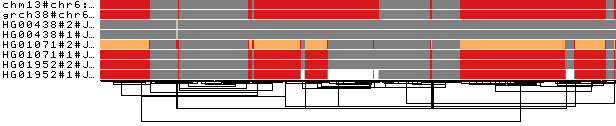
\includegraphics[width=1.0\linewidth, trim=-0cm 2cm 0 0cm]{fig/sorting/chr6_pan_fa_a2fb268_4030258_6a1ecc2_smooth_C4_bad_sorted}
		\label{fig:bad-sorting}
	\end{subfigure}
%	\includegraphics[width=\linewidth]{fig/metrics/chr4.pan.HTTex1.gfa.multiqc_odgi_stats.png}
	\caption{
		PLACEHOLDER IMAGE
		XXX XXX XXX
	}
	\label{fig:sorting}
\end{figure}


\section{Results}

We evaluated the performance of wfmash \texttt{90ea671} against Minimap2-v2.20-r1061~\citep{29750242} and
Winnomap 2.03~\citep{XXX}, in terms of runtime and memory usage. The comparison was performed on both simulated
and real datasets. Simulated data allowed evaluating the alignment quality by calculating precision and recall
in variant identification. The evaluations were performed on a workstation running Ubuntu 20.04 equipped with
64 GB of RAM and an Intel i9-9900K CPU with 8 cores (16 threads). All commands are provided in the Supplementary Material.

\subsection{Simulated data}
We simulated long sequences from the \textit{Saccharomyces cerevisiae} chromosome IV (S288C strain) and the
telomere-to-telomere (T2T) assemblies of the human chromosomes 8, at different levels of length and divergence
(\FIXME{MAYBETable 1 and Table 2}). Chromosomes were split into shorter sequences using the splitfa tool (6a0bb67)~\citep{splitfa}.
In each run, all sequences have the same length, with 50\% of them in reverse complement respect to the source
chromosome. Single nucleotide variants~(SNVs), small indels, and structural variants~(SVs) were introduced
using the Mutation-Simulator script~\citep{32780803}.
%, while structural variants (SVs) were applied using the SURVIVOR benchmarking tool~\citep{28117401}.

To evaluate the correctness of the alignments, in each run we used the pairwise alignment of the input sequences to build
a pangenome graph and identify the variants embedded in it. The graphs were built using~\citep{seqwish}.
seqwish implements a lossless conversion from pairwise alignments between sequences to a pangenome graph encoding the
sequences and their alignments. We called SNVs, small indels, and SVs using vg deconstruct~\citep{30125266},
evaluating the false-negative and false-positive rates using vcfeval~\citep{vcfeval} for SNVs and small indels,
and FIXME XXXXX for SVs.

\begin{comment}
\begin{table}[!t]
    \processtable{
        \small
        Performance of pairwise alignment of long sequences from the \textit{Saccharomyces cerevisiae}
        chromosome IV.
        \label{Tab:01}} {
        \begin{tabular}{@{}llllllll@{}}
            \toprule Aligner & Divergence & Length & Runtime (mm:ss) & Memory (GB) & Precision & Sensitivity & F-measure \\
            \midrule
            row1             & row1       & row1   & row1            & row1        & row1      & row1        & row1      \\
            row2             & row2       & row2   & row2            & row1        & row1      & row1        & row1      \\
            row3             & row3       & row3   & row3            & row1        & row1      & row1        & row1      \\
            row4             & row4       & row4   & row4            & row1        & row1      & row1        & row1      \\
            \botrule
        \end{tabular}
    }

\end{table}
\end{comment}

% TODO Simulation with full chromosomes too

% TODO 7 Mbp beta-defensin locus (chr8: 6,300,000-13,300,000): wfmash/minimap2/winnomnap2

% TODO Centromere (chr8:42,881,543-47,029,467): only wfmash

\subsection{Real data}
XXXXX
\\
% Yeast/HPRC data time/memory
% Histogram of the contig length distribution (supplementary?)



\section{Discussion}
We implemented a novel gap-affine pairwise aligner, wfmash, to accelerate the computation of the mutual
alignment of collections of genomes, a step required for constructing pangenome models. We have demonstrated that
it efficiently performs with contigs representing full human chromosomes of 88 phased haplotypes from the
Human Pangenome Reference Consortium year 1 assembly. Indeed, thanks to its efficiency, wfmash is already
successfully applied in our pangenome graphs building pipeline~\citep{pggb}. No less important, pairwise
alignment is a central step of many bioinformatics applications, making our aligner a scalable solution to face the
increasing yields of sequencing technologies in the coming years.

\section*{Acknowledgements}

We thank members of the HPRC Pangenome Working Group for their insightful discussion and feedback, and members of the HPRC production teams for their development of resources used in our exposition.

\section*{Funding}

We gratefully acknowledge support from NIH/NIDA U01DA047638 and NIH/NIGMS R01GM123489 (EG).


\section*{Data availability}

%Data used to build human pangenome graphs: \url{https://github.com/human-pangenomics/HPP_Year1_Data_Freeze_v1.0}. 
%The graphs we generated the figures from: \url{https://s3-us-west-2.amazonaws.com/human-pangenomics/index.html?prefix=pangenomes/scratch/2021_11_04_pggb_wgg.87/}.
Code and links to data resources used to build this manuscript and its figures, can be found in the paper's public repository: \url{https://github.com/AndreaGuarracino/wfmash-paper}.


\bibliographystyle{natbib}
%\bibliographystyle{achemnat}
%\bibliographystyle{plainnat}
%\bibliographystyle{abbrv}
%\bibliographystyle{bioinformatics}
%
%\bibliographystyle{plain}
%
\bibliography{document}


% \begin{thebibliography}{}

% \bibitem[Bofelli {\it et~al}., 2000]{Boffelli03}
% Bofelli,F., Name2, Name3 (2003) Article title, {\it Journal Name}, {\bf 199}, 133-154.

% \bibitem[Bag {\it et~al}., 2001]{Bag01}
% Bag,M., Name2, Name3 (2001) Article title, {\it Journal Name}, {\bf 99}, 33-54.

% \bibitem[Yoo \textit{et~al}., 2003]{Yoo03}
% Yoo,M.S. \textit{et~al}. (2003) Oxidative stress regulated genes
% in nigral dopaminergic neurnol cell: correlation with the known
% pathology in Parkinson's disease. \textit{Brain Res. Mol. Brain
% Res.}, \textbf{110}(Suppl. 1), 76--84.

% \bibitem[Lehmann, 1986]{Leh86}
% Lehmann,E.L. (1986) Chapter title. \textit{Book Title}. Vol.~1, 2nd edn. Springer-Verlag, New York.

% \bibitem[Crenshaw and Jones, 2003]{Cre03}
% Crenshaw, B.,III, and Jones, W.B.,Jr (2003) The future of clinical
% cancer management: one tumor, one chip. \textit{Bioinformatics},
% doi:10.1093/bioinformatics/btn000.

% \bibitem[Auhtor \textit{et~al}. (2000)]{Aut00}
% Auhtor,A.B. \textit{et~al}. (2000) Chapter title. In Smith, A.C.
% (ed.), \textit{Book Title}, 2nd edn. Publisher, Location, Vol. 1, pp.
% ???--???.

% \bibitem[Bardet, 1920]{Bar20}
% Bardet, G. (1920) Sur un syndrome d'obesite infantile avec
% polydactylie et retinite pigmentaire (contribution a l'etude des
% formes cliniques de l'obesite hypophysaire). PhD Thesis, name of
% institution, Paris, France.

% \end{thebibliography}
\end{document}
